\documentclass{article}

% Language setting
% Replace `english' with e.g. `spanish' to change the document language
\usepackage[english]{babel}

% Set page size and margins
% Replace `letterpaper' with `a4paper' for UK/EU standard size
\usepackage[letterpaper,top=2cm,bottom=2cm,left=3cm,right=3cm,marginparwidth=1.75cm]{geometry}
\usepackage{cite}
% Useful packages
\usepackage{amsmath}
\usepackage{graphicx}
% \usepackage{graphicx}
\usepackage{subcaption}
\usepackage{caption}
\usepackage[colorlinks=true, allcolors=blue]{hyperref}

\title{\textbf{CS 499 - PROJECT COURSE - SEMESTER VII - REPORT 1}}

\author{
  Sameer G Kulkarni\\
  \texttt{sameergk@iitgn.ac.in}
  \and
  Tirth Patel\\
  \texttt{pateltirth@iitgn.ac.in}
  \and
  Mithil Pechimuthu\\
  \texttt{pechimuthumithil@iitgn.ac.in}
  \and
  Sachin Jalan\\
  \texttt{jalansachin@iitgn.ac.in}
}

\begin{document}
\maketitle

\begin{abstract}
The Domain Name System (DNS) protocol has remained unchanged since its inception in 1983. While it is efficient for general computing, the increasing importance and number of edge devices and IoT may reveal that the current DNS protocol implementation can be power-hungry, slow and insecure. We claim that the DNS protocol implementation has inefficiencies that cause overheads in resource-constrained environments, such as IoT devices with limited energy budgets. The project we undertake this semester investigates the inefficiencies of the current DNS protocol implementation and identifies opportunities for optimization. The results show some aspects the implementation could improve through sandboxed packet capture and analysis of DNS traffic from the top 1000 websites.
\end{abstract}

\section{Problem Statement}
An efficient Domain Name System (DNS) protocol that is lean on overheads is required to execute in resource-constrained environments, such as mobile devices and IoT (Internet of Things) systems. Following are the main overheads:
\begin{itemize}
    \item \textbf{Latency:} DNS resolution can introduce significant latency due to its recursive and iterative querying mechanism. DNS queries are handled sequentially and can result in unnecessary delays. This delay can be a deal breaker in many cases.
    \item \textbf{Scalability:} The DNS protocol works well for general computing and large networks. However, in the context of IoT, the density of devices exceeds a million per kilometre. Given the sequential nature of DNS resolution and low TTL values, such a high number of devices performing DNS resolutions can congest the network.
    \item \textbf{Security:} DNS is vulnerable to spoofing, DoS and poisoning attacks. These issues become critical in IoT ecosystems, where breaches can compromise sensitive data and disrupt operations.
    \textbf{Power:} Each of the above overheads causes the device to consume much power for DNS resolution. Such an overhead is a huge no-no for power-constrained devices.
\end{itemize}
Thus, the current implementation of the DNS protocol needs improvements, necessitating a re-evaluation of how DNS queries are handled and how optimizations can be applied to reduce inefficiencies.

\section{Objectives of the work}
This project aims to recognise, diagnose, and address the inefficiencies in the current DNS protocol implementation by making some substitutions. Specifically, this project aims to:
\begin{itemize}
    \item \textbf{Analyse:} Conduct a thorough analysis of DNS traffic using sandboxed packet capture to identify patterns and inefficiencies. By focusing on DNS requests made to the top 1000 websites, we can gain insights into the common types of DNS queries and their associated overhead.
    \item \textbf{Identify:} Explore opportunities to streamline DNS query processing, such as issuing multiple related queries simultaneously (e.g., querying for NS, A, and AAAA records in one request) or implementing intelligent caching mechanisms that minimise redundant queries.
    \item \textbf{Substitute:} We will propose appropriate solutions for each optimisation opportunity with a proof of concept.
\end{itemize}

\section{Introduction}
The Domain Name System (DNS) is a naming system that translates human-readable domain names, like "iitgn.ac.in," into IP addresses like 72.1.241.188, that machines use to address each other. Usually, all of the DNS operates using a recursive query mechanism, where a DNS resolver iteratively queries multiple DNS servers to resolve a domain name, starting from the root servers (contain info about .com, in, etc...) through the top-level domain (TLD) servers (provide .com, .in,  etc...), and down to the authoritative servers. While the protocol supports issuing multiple queries simultaneously, current implementations typically handle one query at a time, leading to inefficiencies, especially when resolving domains where more than one query is necessary. For example, for iitgn.ac.in alone, we have 38 queries to multiple domains like px.ads.linkedin.com, www.facebook.com, www.googletagmanager.com, cdnjs.cloudflare.com. Also, we can see some common patterns. For instance, when a DNS query requests an NS (Name Server) record for a domain, it is common for  A or AAAA record queries after NS record query. We can do this together, too, and optimise the process.

\section{Experiment Methodology}
\textbf{Note:} All scripts can be found in this \hyperlink{https://github.com/SachinJalan/DNS-Renaissance/tree/main}{Github Repository}. \\
To analyze DNS overhead, we performed studies on the top 1000 websites from cloudflare. We used Docker container to sandbox our test environment as it will prevent in OS level network traffic to interfere with our packet capture.

\subsection{Capturing the packets}
Setup a Docker container and used the following tools:
\begin{itemize}
    \item \texttt{dumpcap} for packet capture over the interface \texttt{eth0}.
    \item \texttt{wget} for downloading website content.
\end{itemize}
Using \texttt{wget} a script downloaded the content of the landing page for each website. The \texttt{wget} command was executed with specific flags to ensure DNS data was not cached and only fresh queries were performed \cite{wget}:
\begin{verbatim}
wget --no-dns-cache --no-verbose --timeout 10 -t 1 -c -E -H -k -K -p https://www.iitgn.ac.in
\end{verbatim}

\subsection{Packet Analysis}
The captured packets (stored in \texttt{.pcapng} format) were analyzed using a custom Python script using \textbf{python-pcapng}. For each website, the script extracted the following parameters:
\begin{itemize}
    \item \textbf{Total Packets}: The total number of packets captured.
    \item \textbf{Total Bytes}: The total bytes of data exchanged.
    \item \textbf{Total DNS Packets}: The total number of DNS-specific packets.
    \item \textbf{Total DNS Bytes}: The total bytes of DNS-related traffic.
    \item \textbf{Total Time}: The total duration for complete page load.
    \item \textbf{Total DNS Time}: The total duration for DNS resolution.
    \item \textbf{Time to First Byte (TTFB)}: The time taken to receive the first byte of the response.
    \item \textbf{Total DNS Cycles}: The number of CPU cycles used during DNS resolution using the \texttt{perf} tool.
    \item \textbf{Total DNS Energy}: The energy consumption during DNS resolution, captured using the \texttt{perf} tool.
    \item \textbf{Visited Domains}: A list of all the domains involved in the page load with there respective record types.
\end{itemize}

\subsection{Data Visualization and Analysis}
After extracting the relevant information from the packet captures, we used another Python script to visualize the data. The captured data was plotted to highlight trends and patterns related to DNS overhead across the top 1000 websites. These insights formed the basis for further analysis, which will be detailed in the results section.

\section{Results}
Please find the plots that show the results of the experiment at the end of the document.

% \begin{figure}[htpb]
%     \centering
%     \vspace{-3mm}
%     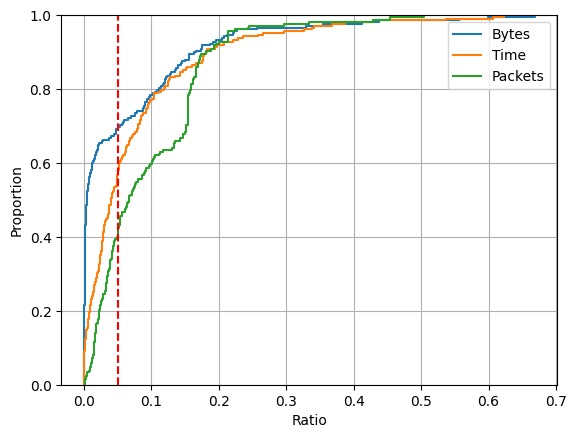
\includegraphics[width=\linewidth]{plots/ratio-bytes-time.jpeg}
%     \vspace{-7mm}
%     \caption{This shows the CDF of the ratio of byte, time taken, and packets involved in DNS resolution. The 5\% critical region is also marked. From this, we infer that 60\%, 40\%, and 35\% of websites are beyond the 5\% limit.}
%     \vspace{-3mm}
%     \label{fig:ratio-bytes-time}
% \end{figure}

\begin{figure}[htpb]
    \centering
    \begin{subfigure}[b]{0.48\linewidth}
        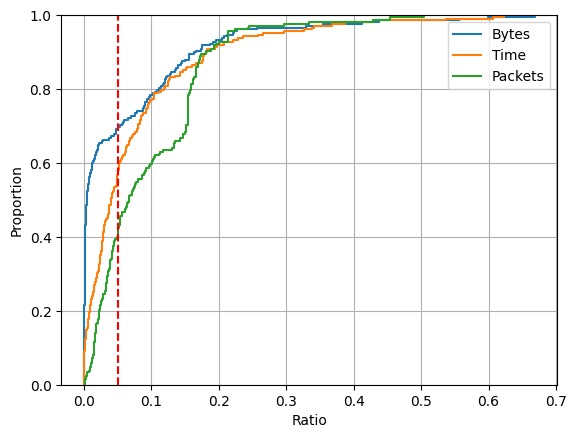
\includegraphics[width=\linewidth]{plots/ratio-bytes-time.jpeg}
        \vspace{-7mm}
        \caption{This shows the CDF of the ratio of byte, time taken, and packets involved in DNS resolution. The 5\% critical region is also marked. From this, we infer that 60\%, 40\%, and 35\% of websites are beyond the 5\% limit.}
        \vspace{-3mm}
        \label{fig:ratio-bytes-time}
    \end{subfigure}
    \hfill
    \begin{subfigure}[b]{0.48\linewidth}
        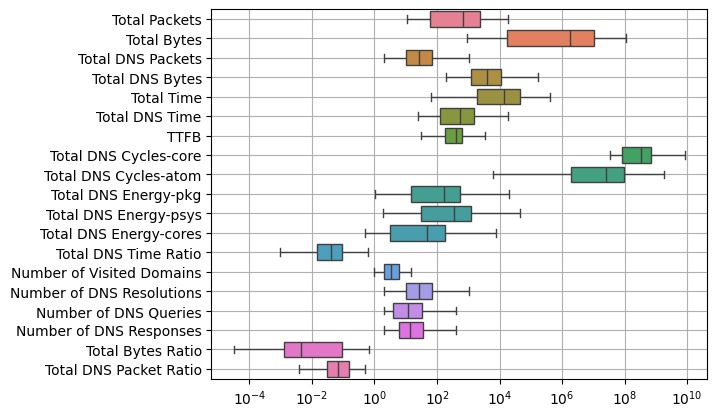
\includegraphics[width=\linewidth]{plots/overall-candle.jpeg}
        \vspace{-7mm}
        \caption{Variation and statistical values of all the parameters calculated.}
        \vspace{-3mm}
        \label{fig:packet-ratio}
    \end{subfigure}
\end{figure}


\begin{figure}[htpb]
    \centering
    \begin{subfigure}[b]{0.48\linewidth}
        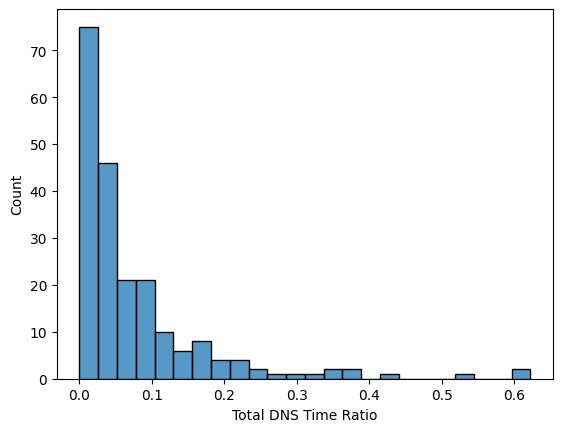
\includegraphics[width=\linewidth]{plots/time-ratio.jpeg}
        \vspace{-7mm}
        \caption{A histogram plot of the number of websites (out of 1000) vs the ratio of time taken for DNS resolution. This supplements Fig.~\ref{fig:ratio-bytes-time}.}
        \vspace{-3mm}
        \label{fig:time-ratio}
    \end{subfigure}
    \hfill
    \begin{subfigure}[b]{0.48\linewidth}
        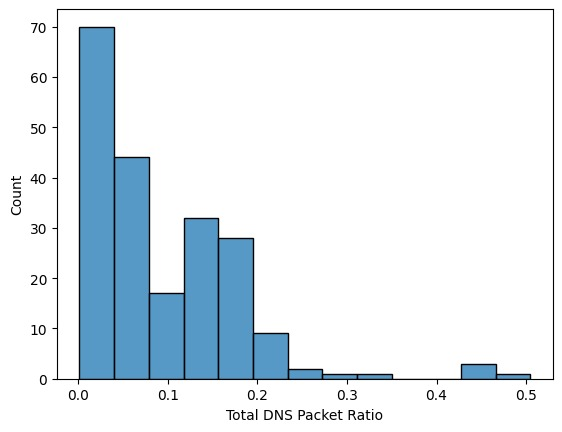
\includegraphics[width=\linewidth]{plots/packet-ratio.jpeg}
        \vspace{-7mm}
        \caption{A histogram plot of the number of websites (out of 1000) vs the ratio of packets involved in DNS resolution out of all packets. This supplements Fig.~\ref{fig:ratio-bytes-time}.}
        \vspace{-3mm}
        \label{fig:packet-ratio}
    \end{subfigure}
\end{figure}

\begin{figure}[htpb]
    \centering
    \begin{subfigure}[b]{0.48\linewidth}
        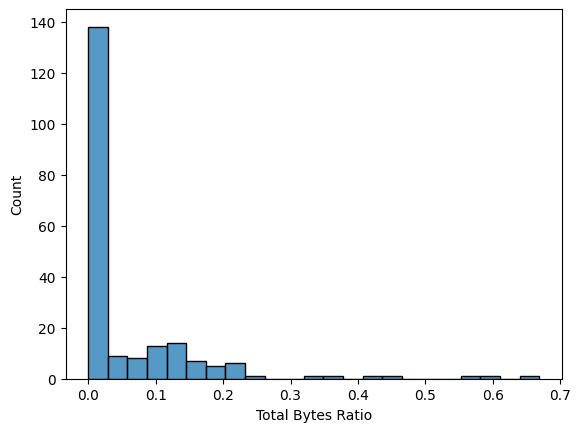
\includegraphics[width=\linewidth]{plots/bytes-ratio.jpeg}
        \vspace{-7mm}
        \caption{A histogram plot of the number of websites (out of 1000) vs the ratio of bytes consumed for DNS resolution out of all bytes for the complete page load. This supplements Fig.~\ref{fig:ratio-bytes-time}.}
        \vspace{-3mm}
        \label{fig:bytes-ratio}
    \end{subfigure}
    \hfill
    \begin{subfigure}[b]{0.48\linewidth}
        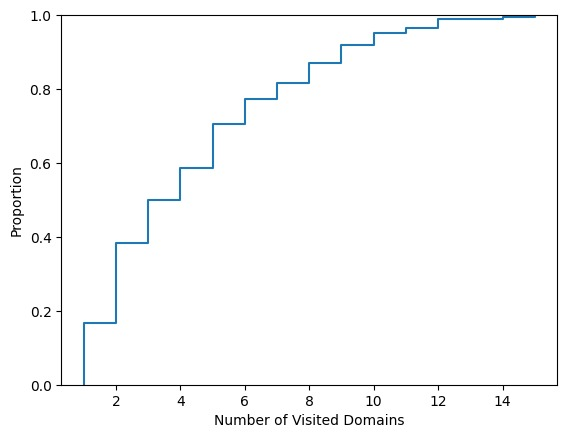
\includegraphics[width=\linewidth]{plots/visited-cdf.jpeg}
        \vspace{-7mm}
        \caption{A CDF plot of the proportion of websites vs the number of domains they visit.}
        \vspace{-3mm}
        \label{fig:visited-cdf}
    \end{subfigure}
\end{figure}

\begin{figure}[htpb]
    \centering
    \begin{subfigure}[b]{0.48\linewidth}
        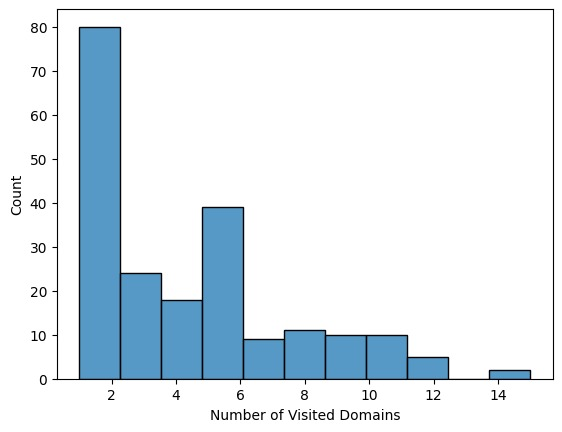
\includegraphics[width=\linewidth]{plots/visited-hist.jpeg}
        \vspace{-7mm}
        \caption{A histogram plot of the count of websites vs the number of domains they visit.}
        \vspace{-3mm}
        \label{fig:visited-hist}
    \end{subfigure}
    \hfill
    \begin{subfigure}[b]{0.48\linewidth}
        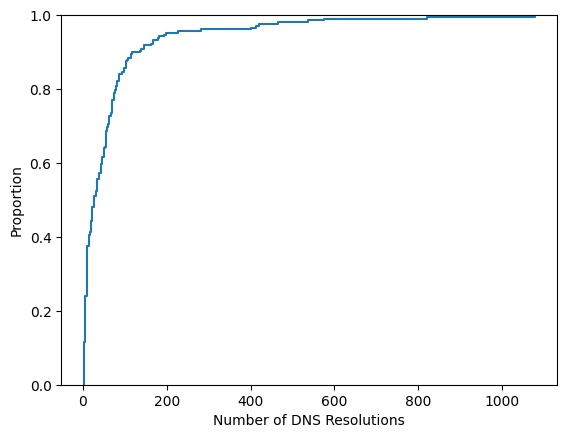
\includegraphics[width=\linewidth]{plots/num-res-cdf.jpeg}
        \vspace{-7mm}
        \caption{A CDF plot of the proportion of websites (out of the 1000) vs the number of DNS resolutions done.}
        \vspace{-3mm}
        \label{fig:num-res-cdf}
    \end{subfigure}
\end{figure}

\begin{figure}[htpb]
    \centering
    \begin{subfigure}[b]{0.48\linewidth}
        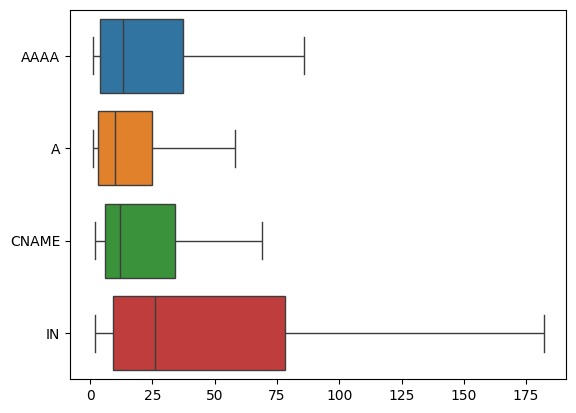
\includegraphics[width=\linewidth]{plots/records-box.jpeg}
        \vspace{-7mm}
        \caption{Amortized counts of the various record types and classes queried for.}
        \vspace{-3mm}
        \label{fig:records-box}
    \end{subfigure}
    \hfill
    \begin{subfigure}[b]{0.48\linewidth}
        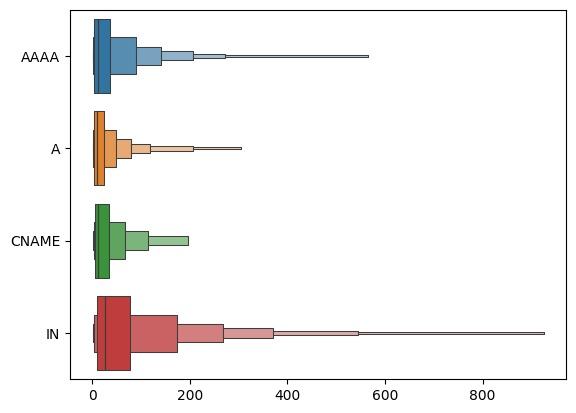
\includegraphics[width=\linewidth]{plots/records-boxen.jpeg}
        \vspace{-7mm}
        \caption{Amortized counts of the various record types and classes queried for.}
        \vspace{-3mm}
        \label{fig:records-boxen}
    \end{subfigure}
\end{figure}

\begin{figure}[htpb]
    \centering
    \vspace{-3mm}
    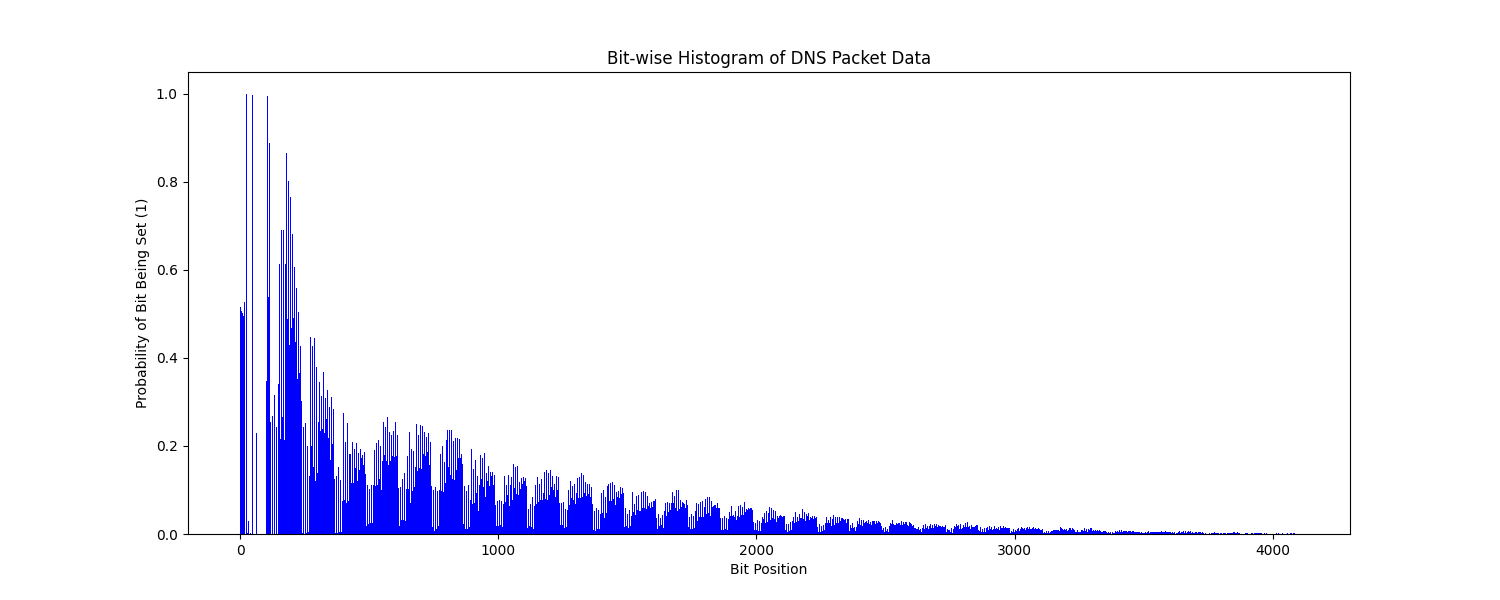
\includegraphics[width=\linewidth]{plots/bits-hist.png}
    \vspace{-7mm}
    \caption{For multiple DNS queries we analyse (assuming max packet size as 512 bytes) the bits of the DNS packets. We plot the probability of a bit being set to 1 from the DNS packets captured from top 1000 websites. We see that many bits have a very low chance of being set to 1. Many bits are also not utilized. There are exactly 67 not utilized bits. For example in case of QDCOUNT field in the header which occupies bits positions 33 to 47, only the 47th bit is ever utilized, rest are never utilized.}
    \vspace{-3mm}
    \label{fig:overall-candle}
\end{figure}
\section{Literature Survey and Related Work}

We use protocols such as DNS-over-HTTPS to address the security and vulnerabilities of the DNS. An empirical study by Böttger et al. \cite{dns-over-https} investigates the costs associated with DoH in terms of performance impact, revealing that while the implementation of DoH adds overhead due to additional security layers, this impact on web page load times is minimal. The study compares DoH to its predecessor, DNS-over-TLS (DoT), and traditional UDP-based DNS, highlighting that DoH offers advantages such as improved privacy without severely compromising performance. However, this work did not cover the other metrics of DNS in the manner we required. It necessitated us to perform our experiments.

While searching to address the DNS protocol's overheads, we came across "CoDNS: Improving DNS Performance and Reliability via Cooperative Lookups," \cite{codns} which explores innovative approaches to DNS by employing cooperative querying techniques to enhance resolution speed and reliability across networks. This method contrasts with conventional DNS lookups, providing insights into performance optimisations that facilitate more efficient DNS handling in dynamic environments. However, this work looks into a different approach to reduce the DNS lookup times using a trusted group of nodes. It involves security issues, too.

Another work, The "Flare-DNS Resolver (FDR) for optimising DNS lookup overhead in mobile devices" \cite{flare-dns} adds to this body of work by focusing specifically on mobile environments. This resolver optimises DNS queries to reduce latency, which is particularly crucial in mobile contexts where network conditions can be highly variable. The contributions of FDR further underline the necessity for dedicated solutions that cater to the unique challenges faced by mobile DNS resolution. It thoroughly analyses the effect of current DNS implementation on DNS lookup times on mobile devices. Moreover, it addresses the issue that an application generally makes multiple DNS resolutions that can be resolved in advance instead of having them staggered. 

% \section{Next Steps} 
% \begin{itemize}
%     \item The above analysis was performed on laptops. The next analysis can be performed on mobile and edge devices. 
%     \item Address and come up with solutions to have multiple queries answered in a single DNS transaction.
%     \item Analyse certain patterns to rebuild the DNS protocol to change certain aspects.
% \end{itemize}

\section{Recent Update}
\begin{figure}[htpb]
    \centering
    \begin{subfigure}[b]{0.48\linewidth}
        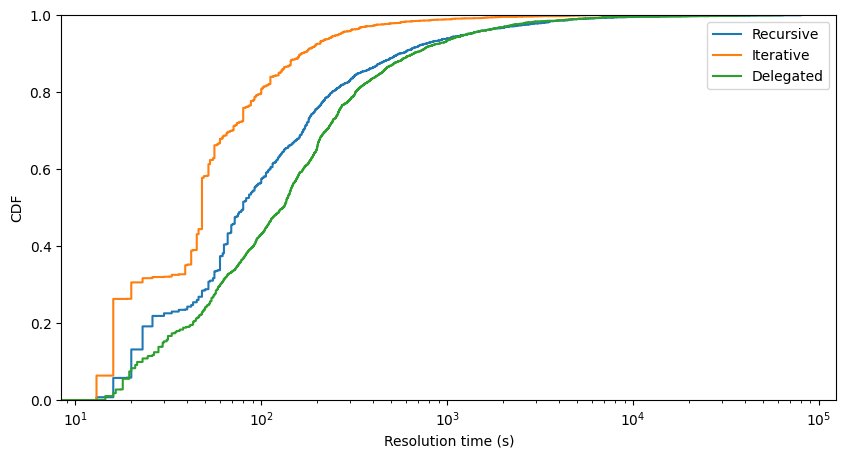
\includegraphics[width=\linewidth]{plots/rec-iter-del-cdf.png}
        \vspace{-7mm}
        \caption{CDF plot for recursive, iterative and delgation mode of DNS resolution.}
        \vspace{-3mm}
        \label{fig:records-box}
    \end{subfigure}
    \hfill
    \begin{subfigure}[b]{0.48\linewidth}
        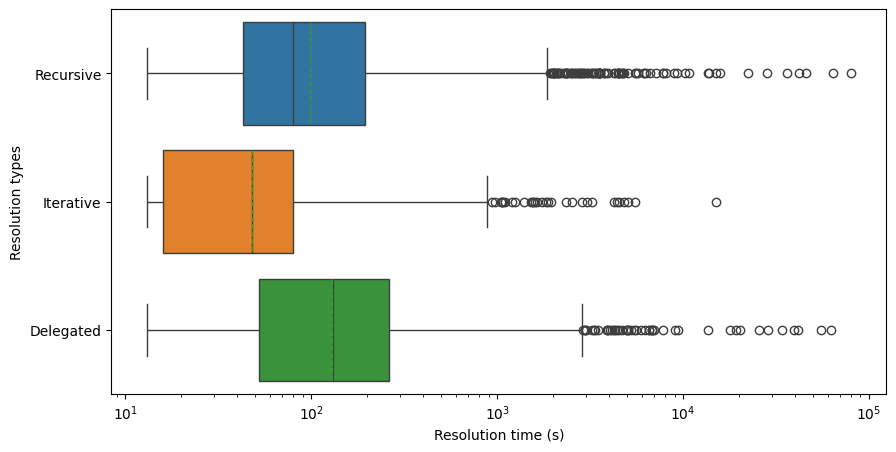
\includegraphics[width=\linewidth]{plots/rec-iter-del-boxplot.png}
        \vspace{-7mm}
        \caption{Box plots for recursive, iterative and delgation mode of DNS resolution.}
        \vspace{-3mm}
        \label{fig:records-boxen}
    \end{subfigure}
\end{figure}

\begin{itemize}
    \item 0.3\% of the total (17277) DNS queries needed to be shifted to TCP through UDP. Most of these queries were for the AAAA record. This shift to TCP causes about 1.5x increase in DNS resolution time.
    \item It must also be noted that A and AAAA records are the only requested records observed for the top 1000 websited. Along with this, CNAME records were present in the answer of some A, AAAA record requests for certain domains.
    \item Around 5\% of the DNS requests encountered benefited from delegating the name server to return the answer to the client.
    \item Almost 7 bytes corresponding to the aa, z, qdcount, nscount, arcount fields in the DNS header were never used in the page load of the top 1000 websites.
\end{itemize}
% \section{Timeline}
% We propose to get things done as follows:
% \begin{itemize}
% \end{itemize}

% \section{Appendix A: Our Efforts}

\bibliographystyle{plain}
\bibliography{sample}

\end{document}